\subsection{Reverse-engineering устройства}

Для того, что бы разработать эмулятор устройства необходимо понять что оно из себя представляет и по какому принципу работает. Первый этап -- визуальный осмотр. Модуль светодиодного экрана представляет из себя алюминиевый каркас, где расположены следующие элементы:
\begin{itemize}
    \item Блок питания;
    \item Принимающая сигнал от контроллера плата;
    \item Индикация состояния модуля;
    \item 4 субмодуля (светодиодные матрицы).
\end{itemize}

Интерфейс подключения матрицы к модулю состоит из нескольких пар RGB, неизвестных контактов, обозначенных как ABCDE, питания, CLK, OE, LAT.

Первым делом была принята попытка подать напряжение на группы RGB, но реакции не последовало. Грустно. Далее, при помощи подключенного к контактам модуля логического анализатора был снят дамп изменений уровней при подаче разного видеосигнала на вход контроллера экрана.
\begin{figure}[ht]
    \centering
    \includegraphics[width=0.9\linewidth]{\commonSecPathPrefix/sec_6/content/analizer.jpg}
    \caption{Графики изменения сигналов на контактах субмодуля}
\end{figure}

Для лучшего понимания принципа работы, был проведен поиск принципа работы светодиодных матриц в целом, без привязки к тематике светодиодных экранов. В результате нещадного протирания клавиатуры и поиска информации на Reddit\cite{reddit}, была обнаружена структурная схема подобных светодиодных матриц.

\begin{figure}[ht]
    \centering
    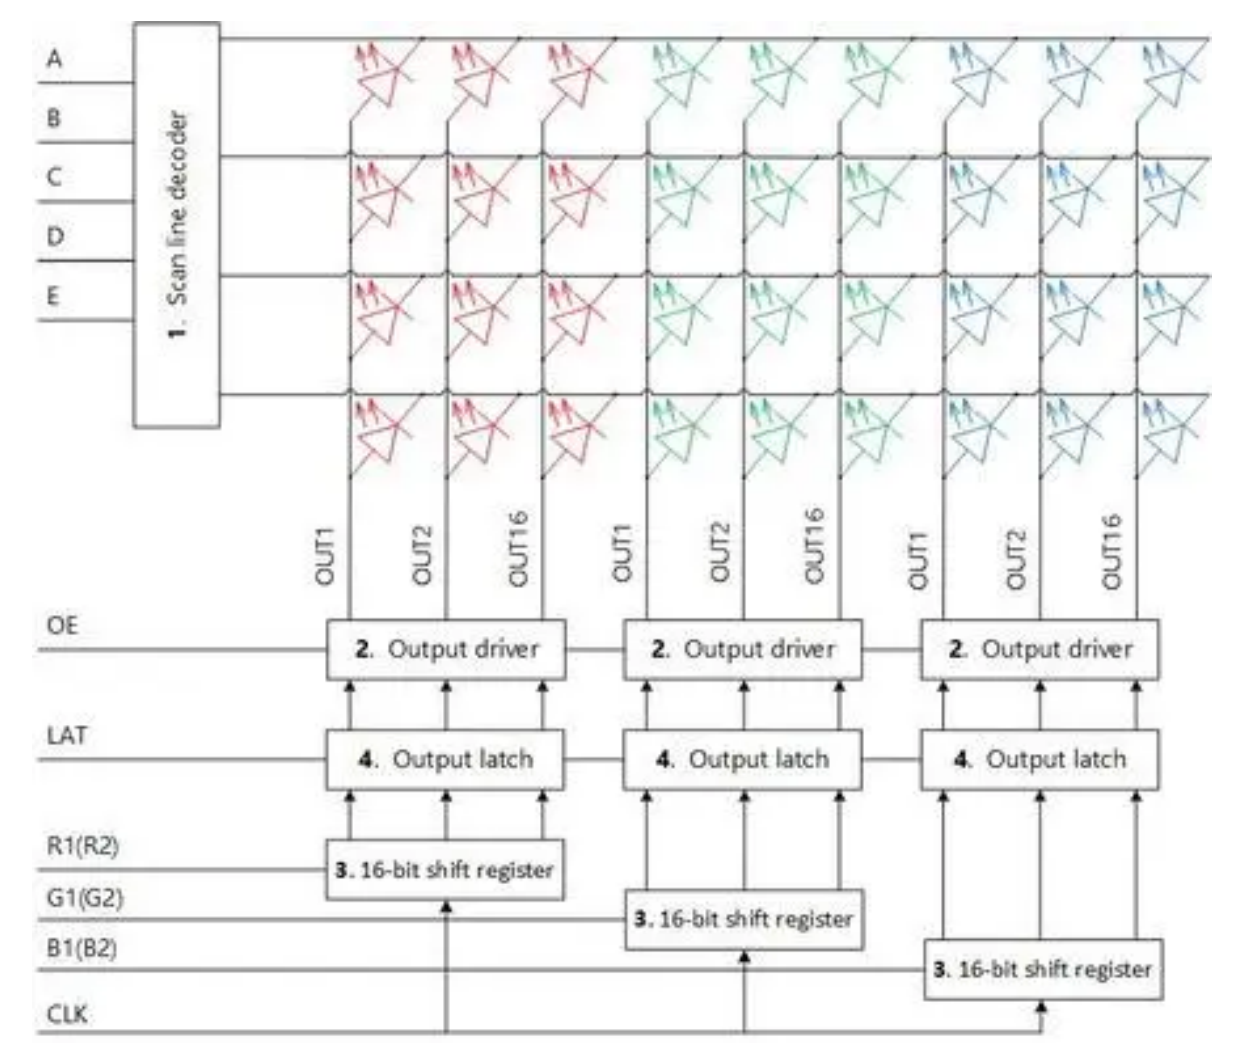
\includegraphics[width=0.8\linewidth]{\commonSecPathPrefix/sec_6/content/led_matrix_structure.png}
    \caption{Структурная схема матрицы}
\end{figure}

После этого принцип работы стал понятен и, используя данные о контактах нескольких типов светодиодных экранов, был определен алгоритм работы такого рода индикации.